% ============================================================================
% Trustilo - AIF Project Requirement + Literature Review Submission
% Generated from the supplied Trustilo proposal and the AIF requirement /
% literature-review templates.  Research gaps were supplemented with primary
% academic and standards sources current to August 2026.
% Compile with pdfLaTeX.  References are embedded via thebibliography.
% ============================================================================
\documentclass[11pt,journal,onecolumn]{IEEEtran}
\IEEEoverridecommandlockouts

\usepackage[letterpaper,margin=0.72in]{geometry}
\usepackage{float}
\usepackage{cite}
\usepackage{amsmath,amssymb}
\usepackage{graphicx}
\usepackage{textcomp}
\usepackage{xcolor}
\usepackage{tikz}
\usetikzlibrary{arrows.meta,shapes.geometric,positioning,fit,backgrounds,calc,shadows}
\usepackage{pgfgantt}
\usepackage{booktabs,multirow,array,tabularx,longtable}
\usepackage{pdflscape}
\usepackage{enumitem}
\usepackage{xurl}
\usepackage[hidelinks]{hyperref}
\hypersetup{breaklinks=true}

\setlength{\parskip}{0.25em}
\setlength{\parindent}{1em}
\renewcommand{\arraystretch}{1.18}
\newcolumntype{Y}{>{\raggedright\arraybackslash}X}
\newcolumntype{L}[1]{>{\raggedright\arraybackslash}p{#1}}

% restrained palette
\definecolor{orchcolor}{RGB}{40,60,110}
\definecolor{intakecolor}{RGB}{225,238,250}
\definecolor{retrievalcolor}{RGB}{222,245,236}
\definecolor{draftcolor}{RGB}{255,241,214}
\definecolor{verifycolor}{RGB}{252,224,224}
\definecolor{mapcolor}{RGB}{233,224,247}
\definecolor{escalatecolor}{RGB}{255,229,204}
\definecolor{learncolor}{RGB}{224,242,255}
\definecolor{storecolor}{RGB}{235,235,235}
\definecolor{outputcolor}{RGB}{223,246,221}
\definecolor{borderline}{RGB}{70,70,70}

\begin{document}

\title{Trustilo: A Multi-Agent AI System for Automated Security\\Questionnaire Response and Compliance Assurance}
\author{\IEEEauthorblockN{Utsav Acharya, Prashansa Shrestha, Nitesh Baniya}}
\maketitle

\begin{abstract}
Trustilo is a proposed multi-agent AI system for automating security-questionnaire response while preserving evidence traceability and human oversight. The system ingests security and infrastructure questionnaires, retrieves supporting material from a customer-specific versioned knowledge library, drafts evidence-grounded responses, verifies claims and evidence freshness, estimates confidence, and escalates uncertain or contradictory answers to a human reviewer. This report restructures the original proposal to satisfy the supplied AIF Project Requirement and Literature Review templates. It adds explicit stakeholder, functional, and non-functional requirements with measurable success criteria; a data-acquisition and benchmarking plan; a research question and sub-problem breakdown; detailed reviews of nine relevant papers; a literature-review matrix; a baseline and ablation plan; and an updated solution architecture. The MVP deliberately prioritizes the core grounding--verification--escalation loop. Full compliance mapping, risk scoring, portal integrations, multilingual support, and enterprise SSO remain post-MVP extensions.
\end{abstract}

\begin{IEEEkeywords}
multi-agent systems, retrieval-augmented generation, security questionnaires, governance risk and compliance, hallucination detection, RAG evaluation, human-in-the-loop AI
\end{IEEEkeywords}

% ============================================================================
\section{Project Context}
% ============================================================================

\subsection{Project Summary}
Security and governance, risk, and compliance (GRC) teams repeatedly answer customer and vendor security questionnaires using information distributed across policies, audit reports, prior questionnaires, architecture documents, and subject-matter experts. Trustilo aims to reduce this repetitive work through a controlled multi-agent pipeline. Rather than allowing one language model to answer directly from memory, each question is parsed and classified, matched to customer-approved evidence, drafted with citations, checked by a verifier, and either finalized or escalated for human review. The intended result is faster questionnaire completion without sacrificing the evidence trail required for high-stakes security representations.

\subsection{Problem Statement}
The project addresses the following practical problem:

\begin{quote}
\emph{How can security questionnaires be answered substantially faster while ensuring that every material claim is supported by current, customer-approved evidence and that uncertain answers are reliably routed to a human reviewer?}
\end{quote}

Manual questionnaire response is accurate when performed by knowledgeable staff but is slow and repetitive. A direct LLM can generate fluent answers rapidly but may introduce unsupported or stale claims. RAG improves access to external knowledge and provenance \cite{lewis2020rag}, yet retrieval errors and generation inconsistency remain failure modes; later RAG work explicitly adds verification and query revision to address them \cite{he2024covrag}. Trustilo therefore treats questionnaire response as a sequence of separately testable tasks rather than a single generation call.

\subsection{Project Goals}
The project has the following goals:
\begin{enumerate}[leftmargin=1.7em]
    \item Ingest common questionnaire formats and normalize them into individually trackable questions.
    \item Build a customer-specific, versioned knowledge library containing approved evidence and prior responses.
    \item Retrieve the most relevant evidence for each question using hybrid retrieval and re-ranking.
    \item Draft answers that are explicitly constrained to the retrieved evidence and cite the evidence used.
    \item Verify answer--evidence consistency, evidence freshness, and contradictions with prior approved responses.
    \item Produce a calibrated confidence/risk signal and escalate answers that are low-confidence, novel, contradictory, or insufficiently supported.
    \item Measure answer quality, groundedness, retrieval quality, escalation quality, latency, cost, and human-review effort against simpler baselines.
    \item Preserve a clear path to post-MVP compliance-framework mapping, risk scoring, continual learning, vendor-portal integrations, and enterprise access control.
\end{enumerate}

\subsection{Application Areas}
Primary application areas are:
\begin{itemize}[leftmargin=1.7em]
    \item customer security reviews during B2B sales and procurement;
    \item vendor and third-party security assessment preparation;
    \item cloud-security questionnaires such as the Cloud Security Alliance CAIQ;
    \item reuse of security-policy, audit, and control evidence across repeated questionnaires;
    \item post-MVP support for compliance mapping and third-party risk management workflows.
\end{itemize}

\subsection{Project Justification}
The latest CSA Cloud Controls Matrix (CCM) v4.1 contains 207 controls across 17 domains, while its accompanying CAIQ contains 283 assessment questions; CAIQ-Lite still contains 138 questions across the same 17 domains \cite{csa2026ccm,csa2026lite}. This illustrates the volume and structure of standardized cloud-assurance work alone, before organization-specific questionnaires are considered. Trustilo is justified when repeated answers can be reused only if their evidence remains current and when automation must expose provenance rather than merely generate plausible text. RAG provides a foundation for evidence-based generation \cite{lewis2020rag}; compliance-specific RAG research also shows that structured retrieval and reasoning can improve automated compliance checking \cite{sun2025compliance}.

\subsection{Scope}
\textbf{MVP in scope:}
\begin{itemize}[leftmargin=1.7em]
    \item security and infrastructure questions in PDF, XLSX/CSV, or plain-text form;
    \item manual upload of customer-approved policies, architecture/security documents, prior approved answers, SOC-style evidence extracts, and penetration-test summaries;
    \item Orchestrator, Intake/Classification, Retrieval, Drafting, Verification, Escalation, and lightweight Reviewer Console;
    \item evidence-linked answer output, confidence/risk status, and full processing trace;
    \item evaluation on public questionnaire templates plus synthetic/de-identified knowledge documents and SME-labelled test cases.
\end{itemize}

\textbf{Post-MVP / out of scope for initial implementation:}
\begin{itemize}[leftmargin=1.7em]
    \item production-grade privacy/legal drafting and legal advice;
    \item full ISO/IEC 27001, SOC 2, GDPR, HIPAA, and NIST control mapping as an automated decision layer;
    \item third-party risk scoring of external vendors;
    \item live bidirectional integrations with questionnaire portals;
    \item multilingual questionnaires;
    \item enterprise SSO/SAML, advanced RBAC, and regional production deployments;
    \item autonomous model fine-tuning from reviewer edits without a curated approval process.
\end{itemize}

\subsection{Limitations and Constraints}
\begin{itemize}[leftmargin=1.7em]
    \item Real completed questionnaires and internal security evidence are confidential, so early evaluation must rely heavily on public templates, synthetic documents, and explicitly permissioned pilot data.
    \item Ground-truth answer quality requires security/GRC expertise; annotation cost may limit the size of the gold test set.
    \item PDF tables, spreadsheets, scanned documents, and inconsistent questionnaire formatting create ingestion errors that are independent of the language model.
    \item RAG can fail when relevant evidence is absent or not retrieved; verification can also produce false confidence. Human escalation therefore remains a core safety mechanism.
    \item Standards and customer evidence change over time; all evidence must be versioned and carry source/freshness metadata.
    \item Model/API cost, rate limits, and latency constrain how many self-checking or verification calls can be run per question.
    \item The planned academic-project schedule is 24 weeks; features that do not directly validate the core hypothesis are deferred.
\end{itemize}

\subsection{Assumptions}
\begin{itemize}[leftmargin=1.7em]
    \item Users have legitimate access to the questionnaires and evidence they upload.
    \item Pilot data is synthetic, de-identified, or shared with explicit permission.
    \item A security/GRC reviewer is available to create a small gold-standard evaluation set and adjudicate ambiguous cases.
    \item The MVP is English-first and can use hosted LLM APIs; a local model is optional rather than required.
    \item The tool assists questionnaire preparation and evidence organization; it does not itself certify compliance or replace legal/audit judgment.
    \item Numerical success thresholds in this report are initial project acceptance targets and may be revised after pilot calibration.
\end{itemize}

\subsection{Team Member Details}
\begin{table}[H]
\centering
\caption{Team Member Details}
\begin{tabularx}{\textwidth}{L{0.27\textwidth}YY}
\toprule
\textbf{Name} & \textbf{Email ID} & \textbf{GitHub ID} \\
\midrule
Utsav Acharya & clerisy47@gmail.com & clerisy47 \\
Prashansa Shrestha & 079bct056.pawan@pcampus.edu.np & prashansa-shrestha \\
Nitesh Baniya & niteshofficial876@gmail.com & Nitesh-Baniya \\
\bottomrule
\end{tabularx}
\end{table}

% ============================================================================
\section{Requirements}
% ============================================================================

\subsection{Expected Inputs}
\begin{itemize}[leftmargin=1.7em]
    \item Security questionnaires in XLSX/CSV, PDF, or plain text.
    \item Customer-approved evidence documents: security policies, architecture/security descriptions, audit/evidence extracts, penetration-test summaries, and previously approved questionnaire responses.
    \item Evidence metadata: source, owner, version/date, validity period where known, confidentiality label, and document type.
    \item Optional framework metadata for later mapping, e.g. NIST CSF 2.0 categories/subcategories and organization-authorized references.
    \item Human reviewer decisions and corrected answers from pilot runs.
\end{itemize}

\subsection{Expected Outputs}
\begin{itemize}[leftmargin=1.7em]
    \item One proposed response per parsed question, with a processing status.
    \item Evidence citations/snippets and source-document identifiers for every answer claim where evidence exists.
    \item Confidence/risk indicators explaining whether an answer can be accepted automatically or requires review.
    \item Escalation tasks that state the exact concern: missing evidence, contradiction, stale evidence, or verifier disagreement.
    \item Completed questionnaire export where the original format is programmatically writable, plus a separate coverage/confidence report.
    \item Audit trail containing retrieval, draft, verification, human-decision, and final-answer records.
\end{itemize}

\subsection{End-User and Stakeholder Requirements}
\begin{table}[H]
\centering
\caption{End-User and Stakeholder Requirements}
\small
\begin{tabularx}{\textwidth}{L{0.29\textwidth}Y L{0.10\textwidth} Y}
\toprule
\textbf{Requirement / User Story} & \textbf{Details} & \textbf{Priority} & \textbf{Success Criteria} \\
\midrule
As a GRC analyst, I want to upload a questionnaire so that I do not manually copy each question. & Detect question boundaries, IDs, sections, and answer fields from supported formats. & Must & $\geq$95\% of questions in the curated format test set are extracted into the correct row/record. \\
As a GRC analyst, I want proposed answers with evidence so that I can review quickly. & Show answer, cited passage, source, version/date, and status together. & Must & 100\% of auto-finalized answers contain at least one traceable evidence reference. \\
As a security SME, I want only risky items escalated so that I focus on cases needing expertise. & Escalate missing-evidence, contradictory, novel, or low-confidence answers. & Must & Escalation recall $\geq$90\% on SME-labelled ``needs review'' cases. \\
As a reviewer, I want the exact concern highlighted so that I can resolve it without re-reading the full pipeline trace. & Reviewer task includes claim, evidence, verifier result, and suggested correction context. & Must & Reviewer can resolve a flagged answer from one review screen in pilot usability tests. \\
As an auditor/project evaluator, I want answer lineage so that the system is accountable. & Store immutable/versioned question, evidence, draft, verification, human decision, and final output IDs. & Must & 100\% of finalized answers have reconstructable lineage in test audit queries. \\
As a system administrator, I want customer data isolated so that one tenant never retrieves another tenant's evidence. & Tenant/customer namespace filters are applied before retrieval and storage access. & Must & Zero cross-tenant retrievals in adversarial isolation tests. \\
As a project team, we want measurable baselines so that improvements are attributable to the multi-agent design. & Evaluate direct LLM, single-agent RAG, RAG+verification, and full proposed pipeline. & Must & Same held-out dataset and scoring rubric used for every configuration. \\
\bottomrule
\end{tabularx}
\end{table}

\subsection{Functional Requirements}
\begin{table}[H]
\centering
\caption{Functional Requirements}
\small
\begin{tabularx}{\textwidth}{L{0.07\textwidth}L{0.24\textwidth}Y L{0.09\textwidth}Y}
\toprule
\textbf{ID} & \textbf{Requirement} & \textbf{Details} & \textbf{Priority} & \textbf{Success Criteria} \\
\midrule
FR1 & Questionnaire ingestion & Parse PDF, XLSX/CSV, and text into ordered question records while preserving IDs/sections where available. & Must & $\geq$95\% extraction correctness on curated format tests. \\
FR2 & Question classification & Tag domain, question type, answer type, and novelty/duplicate similarity. & Must & $\geq$85\% macro-F1 for domain labels on an SME-labelled subset or an agreed simpler accuracy metric if classes are very small. \\
FR3 & Knowledge ingestion & Chunk, index, version, and tag approved evidence documents. & Must & Every indexed chunk has document ID, version, source, and customer namespace. \\
FR4 & Hybrid retrieval & Retrieve evidence using dense semantic search plus sparse/lexical signals and optional re-ranking. & Must & Evidence Recall@10 $\geq$90\% on the gold retrieval set. \\
FR5 & Grounded drafting & Generate a concise answer only from supplied evidence; return ``insufficient evidence'' when support is absent. & Must & $\geq$95\% claim-support precision for auto-finalized answers. \\
FR6 & Citation generation & Attach passage/document references to material claims. & Must & 100\% of auto-finalized answers include valid traceable citations. \\
FR7 & Verification & Check entailment/support, contradiction, evidence freshness, and consistency against prior approved answers. & Must & Detect $\geq$90\% of deliberately injected unsupported/contradictory test answers. \\
FR8 & Confidence and escalation & Combine retrieval/verifier signals into a confidence/risk decision and create review tasks below threshold. & Must & Needs-review recall $\geq$90\%; precision target $\geq$60\% during pilot. \\
FR9 & Human review & Reviewer can approve, edit, reject, or request evidence and the result becomes the authoritative final response. & Must & All reviewer decisions are persisted and reflected in export. \\
FR10 & Export and report & Export answers and a coverage/confidence report; write back to XLSX where feasible. & Must & No answer/question misalignment in round-trip XLSX tests. \\
FR11 & Feedback capture & Save approved edits as curated examples for later retrieval/reuse. & Should & Approved edit is retrievable by a semantically similar later question. \\
FR12 & Framework mapping & Suggest relevant framework references after answer finalization. & Could / Post-MVP & Mapping precision measured separately before production use; human confirmation required initially. \\
\bottomrule
\end{tabularx}
\end{table}

\subsection{Non-Functional Requirements}
\begin{table}[H]
\centering
\caption{Non-Functional Requirements and Initial Acceptance Targets}
\small
\begin{tabularx}{\textwidth}{L{0.08\textwidth}L{0.20\textwidth}Y L{0.09\textwidth}Y}
\toprule
\textbf{ID} & \textbf{Requirement} & \textbf{Details} & \textbf{Priority} & \textbf{Success Criteria} \\
\midrule
NFR1 & Groundedness & Final auto-approved claims must be supported by cited evidence. & Must & $\geq$95\% claim-support precision on held-out SME review; unsupported-claim rate $\leq$2\% as a stretch target. \\
NFR2 & Security isolation & Protect confidential security documents and prevent cross-customer leakage. & Must & Encryption in transit/at rest in deployment design; zero cross-tenant retrieval in tests. \\
NFR3 & Auditability & Every stage must be reconstructable. & Must & 100\% of finalized answers have question, evidence, draft, verifier, reviewer, and version identifiers. \\
NFR4 & Latency & Automation should be materially faster than manual completion. & Should & Prototype target: 100-question run $<15$ minutes excluding human review under normal API availability. \\
NFR5 & Reliability & A failed agent call must not corrupt unrelated question state. & Must & Idempotent retries; failed stage remains resumable from stored state in fault-injection tests. \\
NFR6 & Usability & Review work should be concentrated on flagged items. & Should & Pilot reviewers can approve/edit without consulting raw logs in $\geq$90\% of flagged cases. \\
NFR7 & Maintainability & Models, retrievers, prompts, and thresholds should be replaceable/configurable. & Should & Configuration/version IDs recorded for each experiment; no hard dependency on one LLM vendor in the domain model. \\
NFR8 & Cost observability & Token/API cost per stage must be measurable. & Should & Cost and latency logged per question and per agent for 100\% of benchmark runs. \\
NFR9 & Explainability & Escalation must state why an answer was flagged. & Must & Every escalated task has at least one machine-readable reason code and a human-readable explanation. \\
\bottomrule
\end{tabularx}
\end{table}

% ============================================================================
\section{Data Collection, Data Sources, and Benchmarking}
% ============================================================================

\subsection{Data Identification}
The project requires four kinds of data:
\begin{enumerate}[leftmargin=1.7em]
    \item \textbf{Question data}: security questionnaire questions, sections, expected answer formats, and domain labels.
    \item \textbf{Evidence data}: policy passages, control descriptions, architecture/security statements, audit evidence summaries, and approved historical answers.
    \item \textbf{Evaluation labels}: evidence-relevance labels, gold answers, claim-support labels, contradiction/staleness flags, and ``needs human review'' labels.
    \item \textbf{Framework metadata}: public or appropriately licensed control/category identifiers and mappings used only for the post-MVP mapping experiment.
\end{enumerate}

\subsection{Data Sources}
\begin{table}[H]
\centering
\caption{Planned Data Sources}
\small
\begin{tabularx}{\textwidth}{L{0.24\textwidth}Y L{0.21\textwidth}}
\toprule
\textbf{Source} & \textbf{Use in Trustilo} & \textbf{Notes} \\
\midrule
CSA CAIQ v4.1 & Main public source of realistic cloud-security questions. & 283 questions aligned to 207 CCM controls across 17 domains \cite{csa2026ccm,csa2026guide}. \\
CSA CAIQ-Lite v4.1 & Smaller benchmark/iteration set. & 138 questions across 17 domains; useful for early end-to-end tests \cite{csa2026lite}. \\
NIST CSF 2.0 & Public framework taxonomy for optional mapping experiments. & Six functions: Govern, Identify, Protect, Detect, Respond, Recover \cite{nist2024csf,nist2024news}. \\
Synthetic customer knowledge base & Provides controlled ground truth without exposing real company secrets. & Team-authored policy/control documents with known facts, versions, and deliberate contradictions/stale versions. \\
Permissioned/de-identified pilot documents & Tests realism after the synthetic benchmark is stable. & Included only with explicit authorization; stored separately from public test data. \\
SME annotations & Gold labels for correctness, evidence support, escalation, and error analysis. & Small, high-quality adjudicated set is preferred over a large weakly labelled set. \\
Research benchmarks & Validate individual RAG/evaluation components. & NQ/WebQ/TriviaQA, WikiEval, PrivacyQA, and compliance datasets are reviewed in Section~\ref{sec:litreview}; they are supporting research evidence, not the primary Trustilo product dataset. \\
\bottomrule
\end{tabularx}
\end{table}

\subsection{Data Acquisition Methods}
\begin{enumerate}[leftmargin=1.7em]
    \item Download public questionnaire/framework artifacts from their official publishers where licensing permits local project use.
    \item Create a synthetic company profile and write internally consistent security-policy/evidence documents with explicit version dates and facts.
    \item Generate question--evidence candidate pairs from CAIQ questions, then manually label a representative subset for retrieval evaluation.
    \item Ask the security/GRC reviewer to create or approve reference answers for a stratified subset of questions spanning major domains.
    \item Create controlled negative cases by removing relevant evidence, inserting contradictory versions, and substituting stale evidence; these cases specifically test verification and escalation.
    \item If a pilot organization participates, ingest only data it explicitly authorizes and de-identify exports used in the academic report.
\end{enumerate}

\subsection{Data Collection Challenges}
Key challenges are confidentiality, limited gold labels, document-format heterogeneity, class imbalance between easy/repeated and novel questions, changes in standards and internal policies, ambiguous questionnaire wording, and the risk that synthetic documents are easier than real enterprise evidence. To reduce benchmark leakage, the final Trustilo test set should be frozen before prompt/threshold tuning and kept separate from development examples.

\subsection{Establishing Baseline Models}
The experiment will use progressively stronger baselines:
\begin{description}[leftmargin=2.1cm,style=nextline]
    \item[B0: Direct LLM] Question only, no external evidence. This is intentionally weak but measures the value of retrieval and exposes unsupported-answer behavior.
    \item[B1: Single-agent RAG] One retriever plus one answer-generation call using retrieved evidence; no independent verification agent.
    \item[B2: RAG + verifier] Same as B1 plus a separate evidence-support/contradiction check, but without multi-agent routing and human escalation logic.
    \item[P: Trustilo] Orchestrated classification + hybrid retrieval + grounded drafting + verification + confidence/escalation + human review.
    \item[Human reference] SME-written/approved answers and fully manual completion time on a small subset, used as a reference rather than as a machine baseline.
\end{description}

\subsection{Resources Required}
\begin{itemize}[leftmargin=1.7em]
    \item \textbf{People}: three project members plus periodic access to at least one security/GRC SME for labelling and adjudication.
    \item \textbf{Compute}: ordinary development machines are sufficient when hosted LLM APIs are used; local embedding/reranking models can run on CPU/GPU depending on the selected model. Local large-model serving is optional.
    \item \textbf{Software}: Python backend, document parsers, relational database, object storage, vector/sparse retrieval stack, agent/state-graph orchestration, web reviewer UI, and experiment-tracking/logging.
    \item \textbf{Data}: CAIQ/CAIQ-Lite, NIST CSF references, synthetic company corpus, and a held-out SME-labelled benchmark.
    \item \textbf{Security}: isolated test storage, access control, secrets management, and redaction rules for any pilot data.
\end{itemize}

% ============================================================================
\section{Literature Review}
\label{sec:litreview}
% ============================================================================

\subsection{High-Level Research Question}
\textbf{RQ:} \emph{Can a multi-agent, retrieval-grounded, verification-and-escalation pipeline answer security questionnaires with higher evidence faithfulness and lower human-review effort than a direct LLM or a single-agent RAG baseline?}

\subsection{Sub-Problems for Deeper Analysis}
\begin{enumerate}[leftmargin=1.7em]
    \item How should heterogeneous questionnaire formats be normalized into atomic questions?
    \item Which retrieval strategy best finds the authoritative evidence for each security question?
    \item How can an LLM be constrained to answer only from retrieved evidence and abstain when evidence is insufficient?
    \item How can hallucinated, contradictory, or stale claims be detected after drafting?
    \item How should retrieval quality, answer faithfulness, answer relevance, and reviewer escalation be evaluated?
    \item Can confidence/escalation thresholds reduce reviewer effort without allowing unsafe answers through?
    \item How should approved human corrections be versioned and reused without propagating outdated answers?
    \item How can final responses later be mapped to compliance frameworks while keeping the mapping auditable?
\end{enumerate}

\subsection{General Review: Major Ideas and Terminology}
\begin{itemize}[leftmargin=1.7em]
    \item \textbf{Retrieval-Augmented Generation (RAG):} combines parametric language-model knowledge with external retrieved passages, improving provenance and updateability \cite{lewis2020rag}.
    \item \textbf{Hybrid retrieval and re-ranking:} combines semantic/dense retrieval with lexical search, then uses a stronger cross-encoder or LLM judge to re-rank a small candidate set. Privacy-policy QA research demonstrates the practical value of retriever ensembles and filtering \cite{parvez2023privacyqa}.
    \item \textbf{Verification after generation:} draft--verify--revise methods such as Chain-of-Verification (CoVe) and CoV-RAG explicitly separate generation from fact checking or query revision \cite{dhuliawala2024cove,he2024covrag}.
    \item \textbf{Self-consistency / black-box hallucination detection:} SelfCheckGPT estimates factuality from inconsistency among multiple samples, showing that black-box verification signals can be stronger than token-probability baselines \cite{manakul2023selfcheckgpt}.
    \item \textbf{RAG evaluation:} RAGAS separates faithfulness, answer relevance, and context relevance \cite{es2024ragas}; ARES adds domain-adapted lightweight judges and prediction-powered inference with a small human-labelled set \cite{saadfalcon2024ares}.
    \item \textbf{Structured compliance reasoning:} recent compliance-checking work combines structured static/dynamic knowledge with retrieval and LLM reasoning, indicating that compliance problems benefit from explicit representations rather than raw semantic matching alone \cite{sun2025compliance}.
    \item \textbf{Iterative refinement:} Self-Refine shows that generator--feedback--refiner loops can improve LLM outputs without additional training, supporting the broader design choice to separate roles even when the same base model is used \cite{madaan2023selfrefine}.
    \item \textbf{Human-in-the-loop escalation:} for Trustilo, abstention is a feature, not a failure. Evidence gaps and verifier uncertainty are routed to an SME rather than converted into unsupported prose.
\end{itemize}

\subsection{Datasets and Public Artifacts Relevant to the Problem}
\begin{table}[H]
\centering
\caption{Datasets / Artifacts Identified in the Review}
\small
\begin{tabularx}{\textwidth}{L{0.23\textwidth}L{0.23\textwidth}Y}
\toprule
\textbf{Dataset / Artifact} & \textbf{Problem Type} & \textbf{Relevance to Trustilo} \\
\midrule
CAIQ v4.1 / CAIQ-Lite & Cloud security assessment questions & Primary realistic questionnaire source for the project; 283 full or 138 Lite questions \cite{csa2026guide,csa2026lite}. \\
PrivacyQA & Privacy-policy question answering & Closest reviewed domain-specific QA dataset showing retrieval/data-augmentation challenges \cite{parvez2023privacyqa}. \\
Natural Questions (NQ), WebQuestions, TriviaQA & Open-domain QA & Common retrieval/generation benchmarks used by RAG and CoV-RAG; useful for validating components, not product claims \cite{lewis2020rag,he2024covrag}. \\
WikiEval & RAG metric evaluation & Human-pairwise evaluation data for faithfulness, relevance, and context relevance in RAGAS \cite{es2024ragas}. \\
KILT / SuperGLUE / AIS subsets & RAG-system evaluation & Used by ARES to test context relevance, faithfulness, and answer relevance with small human-labelled sets \cite{saadfalcon2024ares}. \\
EU2UK, GDPR-13, CONTRACT, CSSCD & Compliance checking & Demonstrate document/sentence-level legal/compliance checking and domain transfer \cite{sun2025compliance}. \\
WikiBio factuality annotations & Hallucination detection & Used by SelfCheckGPT to measure sentence/passage factuality from sampled LLM generations \cite{manakul2023selfcheckgpt}. \\
\bottomrule
\end{tabularx}
\end{table}

\subsection{Common Models and Methods}
The review identifies recurring components that map naturally to Trustilo: DPR or other dense bi-encoder retrievers; BM25/sparse retrieval; BERT/DeBERTa-style classifiers or cross-encoders; BART/decoder LLM generators; instruction-tuned LLMs such as Llama-family models; LLM-as-judge or verifier prompts; iterative query rewriting; synthetic data generation; confidence calibration; and human validation sets. The proposed project is therefore not dependent on inventing a new foundation model; its research contribution is primarily the integration, evaluation, and control logic for a security-questionnaire setting.

\subsection{Major Issues Identified}
\begin{enumerate}[leftmargin=1.7em]
    \item \textbf{Retrieval failure}: a good generator cannot cite evidence that was never retrieved.
    \item \textbf{Retrieval-generation mismatch}: retrieved text may be relevant but not sufficient, or the model may ignore/contradict it \cite{he2024covrag}.
    \item \textbf{Hallucination and unsupported synthesis}: fluent output can contain claims absent from the evidence \cite{manakul2023selfcheckgpt,dhuliawala2024cove}.
    \item \textbf{Evaluation without expensive labels}: fully human evaluation is costly; RAGAS and ARES offer automated signals but should not replace a small expert gold set in a high-stakes domain \cite{es2024ragas,saadfalcon2024ares}.
    \item \textbf{Temporal validity}: security evidence can expire or change even when semantically relevant.
    \item \textbf{Confidentiality}: the highest-value enterprise questionnaire/evidence pairs are usually not public.
    \item \textbf{Ambiguity and one-to-many mappings}: a single security question may rely on multiple documents or map to multiple framework controls.
    \item \textbf{Automation bias}: reviewers may over-trust polished AI output; the UI must foreground sources, uncertainty, and reasons for escalation.
\end{enumerate}

% --------------------------- Detailed paper reviews --------------------------
\subsection{Detailed Paper Reviews}
The AIF guideline requests at least five papers and specific fields for each. Nine papers are reviewed below so that retrieval, verification, evaluation, compliance reasoning, domain QA, and iterative refinement are all covered.

\subsubsection{Paper 1: Retrieval-Augmented Generation for Knowledge-Intensive NLP Tasks}
\begin{description}[leftmargin=3.25cm,style=nextline]
\item[Authors / Year] Patrick Lewis et al., 2020 \cite{lewis2020rag}.
\item[DOI / Link] Conference paper; the NeurIPS proceedings page does not list a DOI. Public paper: \url{https://proceedings.neurips.cc/paper/2020/hash/6b493230-Abstract.html}.
\item[Main idea] Combine a parametric seq2seq generator with a non-parametric dense Wikipedia index. RAG-Sequence uses one latent retrieved document for the generated sequence; RAG-Token may use different documents per token.
\item[Datasets] Natural Questions (NQ), TriviaQA (TQA), WebQuestions (WQ), CuratedTREC (CT), MS MARCO, Jeopardy question generation, and FEVER.
\item[Models] DPR-style neural retriever plus a BART generator; the query encoder and generator are fine-tuned while the document index can remain fixed.
\item[Code] The paper links RAG experiments in Hugging Face Transformers: \url{https://github.com/huggingface/transformers/tree/master/examples/rag}.
\item[Procedure / tricks] Retrieve top-$k$ passages, marginalize over retrieved passages during generation, and jointly optimize retrieval/generation components.
\item[Metrics / results] RAG-Sequence reports exact-match scores of 44.5 on NQ, 56.8 on TQA (68.0 on the TQA-Wiki split), 45.2 on WQ, and 52.2 on CT, outperforming the DPR results shown in the same table on NQ/WQ/CT \cite{lewis2020rag}.
\item[Key learning] External non-parametric memory improves knowledge-intensive generation and provides a clean mechanism for updating knowledge. Trustilo should therefore store customer evidence outside model weights and keep source provenance with every chunk.
\end{description}

\subsubsection{Paper 2: Retrieving, Rethinking and Revising: The Chain-of-Verification Can Improve RAG}
\begin{description}[leftmargin=3.25cm,style=nextline]
\item[Authors / Year] Bolei He et al., 2024 \cite{he2024covrag}.
\item[DOI / Link] DOI: 10.18653/v1/2024.findings-emnlp.607. Public paper: \url{https://aclanthology.org/2024.findings-emnlp.607/}.
\item[Main idea] Add a verification module that scores RAG outputs, judges retrieval/answer quality, revises poor queries, re-retrieves, and rewrites answers. The method explicitly targets both external retrieval errors and internal generation inconsistency.
\item[Datasets] Natural Questions, WebQuestions, Mintaka, and TriviaQA.
\item[Models] Experiments include ChatGLM2-6B, Vicuna-7B/13B, and Llama2-7B/13B backbones; GPT-4 is used in parts of data synthesis/evaluation.
\item[Code] ACL provides a software attachment from the paper page: \url{https://aclanthology.org/2024.findings-emnlp.607/}.
\item[Procedure / tricks] Synthetic positive/negative RAG data, verification criteria for reference correctness/correctness/citation accuracy/truthfulness/bias/conciseness, query revision, re-retrieval, and iterative revision.
\item[Metrics / results] With Llama2-13B, CoV-RAG averages 75.1\% accuracy across NQ/WebQ/Mintaka/TriviaQA versus 73.8\% for the WebGLM configuration shown with the same backbone. CoV-RAG with ChatGLM2-6B averages 72.2\% \cite{he2024covrag}.
\item[Key learning] Verification should be able to change the retrieval query and trigger re-retrieval, not merely judge a finished answer. Trustilo therefore includes a verifier-to-retriever retry path for low-support cases.
\end{description}

\subsubsection{Paper 3: A Compliance Checking Framework Based on Retrieval Augmented Generation}
\begin{description}[leftmargin=3.25cm,style=nextline]
\item[Authors / Year] Jingyun Sun, Zhongze Luo, and Yang Li, 2025 \cite{sun2025compliance}.
\item[DOI / Link] ACL Anthology does not list a DOI for this COLING paper. Public paper: \url{https://aclanthology.org/2025.coling-main.178/}.
\item[Main idea] Combine static factual knowledge, dynamic regulatory/business-process knowledge, and a computational retrieval/reasoning layer. An event-centric graph captures actions and states important in regulations.
\item[Datasets] EU2UK, GDPR-13, CONTRACT, and CSSCD (three English datasets and one Chinese dataset).
\item[Models] ChatGLM3-6B for Chinese and Llama2 for English experiments, together with structured graph retrieval/reasoning.
\item[Code] No public code repository is linked from the ACL Anthology record reviewed for this report.
\item[Procedure / tricks] Static entity/concept/term graphs plus dynamic eventic graphs are fused before the LLM produces compliance judgments with explanations.
\item[Metrics / results] Using Matthews Correlation Coefficient (MCC), the proposed framework scores 0.778 on EU2UK, 0.652 on GDPR-13, 0.730 on CONTRACT, and 0.680 on CSSCD; the paper also reports cross-domain MCC of 0.743/0.603/0.714 from CSSCD to EU2UK/GDPR-13/CONTRACT \cite{sun2025compliance}.
\item[Key learning] Compliance reasoning benefits from explicit structured context and explanations. Trustilo should treat framework mapping as a separately auditable stage rather than burying it inside free-form answer generation.
\end{description}

\subsubsection{Paper 4: RAGAs: Automated Evaluation of Retrieval Augmented Generation}
\begin{description}[leftmargin=3.25cm,style=nextline]
\item[Authors / Year] Shahul Es, Jithin James, Luis Espinosa Anke, and Steven Schockaert, 2024 \cite{es2024ragas}.
\item[DOI / Link] DOI: 10.18653/v1/2024.eacl-demo.16. Public paper: \url{https://aclanthology.org/2024.eacl-demo.16/}.
\item[Main idea] Provide reference-free component metrics for RAG pipelines instead of evaluating only the final answer.
\item[Datasets] WikiEval, constructed for human pairwise comparisons of answer faithfulness, answer relevance, and context relevance.
\item[Models] LLM-based evaluators are used to estimate faithfulness, answer relevance, and context relevance.
\item[Code] \url{https://github.com/explodinggradients/ragas}.
\item[Procedure / tricks] Decompose RAG evaluation into retrieval and generation dimensions and compare automatic metric judgments with human pairwise judgments.
\item[Metrics / results] On WikiEval, reported agreement with human annotators is 0.95 for faithfulness, 0.78 for answer relevance, and 0.70 for context relevance, above the GPT Score and GPT Ranking baselines shown in the paper \cite{es2024ragas}.
\item[Key learning] Trustilo should report retrieval/context quality separately from answer faithfulness. A single ``accuracy'' number hides the stage that failed.
\end{description}

\subsubsection{Paper 5: ARES: An Automated Evaluation Framework for RAG Systems}
\begin{description}[leftmargin=3.25cm,style=nextline]
\item[Authors / Year] Jon Saad-Falcon, Omar Khattab, Christopher Potts, and Matei Zaharia, 2024 \cite{saadfalcon2024ares}.
\item[DOI / Link] DOI: 10.18653/v1/2024.naacl-long.20. Public paper: \url{https://aclanthology.org/2024.naacl-long.20/}.
\item[Main idea] Generate synthetic in-domain training data for lightweight RAG judge models, then use a small human-labelled validation set with prediction-powered inference (PPI) to improve system-level estimates and confidence intervals.
\item[Datasets] Eight knowledge-intensive tasks from KILT, SuperGLUE, and AIS; the paper also tests domain shifts.
\item[Models] DeBERTa-v3-Large is used as the pretrained basis for judge models in the main evaluation; GPT-3.5 is used as a comparison judge.
\item[Code] \url{https://github.com/stanford-futuredata/ARES}.
\item[Procedure / tricks] Synthetic QA generation, separate judges for context relevance/answer faithfulness/answer relevance, contrastive fine-tuning, then PPI using approximately a few hundred human labels.
\item[Metrics / results] ARES averages Kendall's $\tau$ 0.065 higher for context relevance and 0.132 higher for answer relevance than RAGAS in the reported ranking experiments; it also uses 78\% fewer annotations than a sampled-annotation configuration while averaging 0.08 higher $\tau$ across the compared relevance metrics \cite{saadfalcon2024ares}.
\item[Key learning] A small, carefully labelled in-domain validation set can make automated RAG evaluation more useful. Trustilo should budget SME effort for a compact gold set rather than attempting fully label-free evaluation.
\end{description}

\subsubsection{Paper 6: Chain-of-Verification Reduces Hallucination in Large Language Models}
\begin{description}[leftmargin=3.25cm,style=nextline]
\item[Authors / Year] Shehzaad Dhuliawala et al., 2024 \cite{dhuliawala2024cove}.
\item[DOI / Link] DOI: 10.18653/v1/2024.findings-acl.212. Public paper: \url{https://aclanthology.org/2024.findings-acl.212/}.
\item[Main idea] Generate a baseline answer, plan verification questions, answer those questions independently, and produce a revised verified response.
\item[Datasets] Wikidata list questions, QUEST/Wikipedia-category style questions, MultiSpanQA, and long-form generation evaluated for factuality.
\item[Models] Few-shot Llama 65B in the main CoVe experiments, with Llama 2 70B Chat comparisons.
\item[Code] No official code repository is linked from the ACL Anthology record reviewed for this report.
\item[Procedure / tricks] The factored variants prevent verification answers from conditioning directly on the original answer, reducing repetition of the same hallucination.
\item[Metrics / results] In the list-based results, the Llama-65B baseline precision of 0.17 improves to 0.36 with two-step CoVe while average negative/hallucinated entities fall from 2.95 to 0.68 in the corresponding column \cite{dhuliawala2024cove}.
\item[Key learning] Verification should be context-separated from the draft where possible. Trustilo's verifier therefore receives evidence and claims explicitly and should not be instructed simply to ``agree/disagree'' with a persuasive draft.
\end{description}

\subsubsection{Paper 7: SelfCheckGPT: Zero-Resource Black-Box Hallucination Detection}
\begin{description}[leftmargin=3.25cm,style=nextline]
\item[Authors / Year] Potsawee Manakul, Adian Liusie, and Mark Gales, 2023 \cite{manakul2023selfcheckgpt}.
\item[DOI / Link] DOI: 10.18653/v1/2023.emnlp-main.557. Public paper: \url{https://aclanthology.org/2023.emnlp-main.557/}.
\item[Main idea] If an LLM knows a fact, repeated stochastic samples should be relatively consistent; hallucinated facts tend to vary or contradict. This permits black-box hallucination detection without an external database or token probabilities.
\item[Datasets] GPT-3-generated WikiBio passages with manual sentence-level factuality annotations.
\item[Models] GPT-3 generator plus BERTScore, QA, n-gram, NLI, and prompt-based consistency checks.
\item[Code] \url{https://github.com/potsawee/selfcheckgpt}.
\item[Procedure / tricks] Sample multiple outputs (the main analysis uses repeated generations), compare consistency, and aggregate sentence/passage factuality scores.
\item[Metrics / results] SelfCheckGPT-Prompt reaches non-factual AUC-PR 93.42, factual AUC-PR 67.09, Pearson correlation 78.32, and Spearman correlation 78.30 in the paper's main table, outperforming the grey-box GPT-3 probability baseline on those measures \cite{manakul2023selfcheckgpt}.
\item[Key learning] Consistency across samples is a useful auxiliary uncertainty signal, but repeated sampling is expensive. Trustilo may use it selectively only for borderline cases, not for every question.
\end{description}

\subsubsection{Paper 8: Retrieval Enhanced Data Augmentation for QA on Privacy Policies}
\begin{description}[leftmargin=3.25cm,style=nextline]
\item[Authors / Year] Md Rizwan Parvez et al., 2023 \cite{parvez2023privacyqa}.
\item[DOI / Link] DOI: 10.18653/v1/2023.eacl-main.16. Public paper: \url{https://aclanthology.org/2023.eacl-main.16/}.
\item[Main idea] Address extreme positive/negative imbalance in privacy-policy QA by retrieving candidate positive examples from a large unlabeled policy corpus and filtering noisy candidates before augmenting training data.
\item[Datasets] PrivacyQA plus approximately 6.5k crawled privacy-policy documents containing about 0.6M statements for augmentation.
\item[Models] Dense Passage Retriever with BERT/PBERT/SimCSE variants, plus a cross-encoder QA/filtering model.
\item[Code] The paper documents the retrieval/filtering implementation details but does not link a single official project repository in the ACL record reviewed here.
\item[Procedure / tricks] Retriever ensembles, top-$k$ candidate mining, in-batch negatives, filtering/noise reduction, and domain-specific data augmentation.
\item[Metrics / results] The prior BERT+Unanswerable baseline reports F1 39.8. The ensemble-retriever augmentation with filtering (ERA-D) reaches precision 51.0, recall 48.7, and F1 49.8 on PrivacyQA \cite{parvez2023privacyqa}.
\item[Key learning] Domain QA can suffer from scarce positive evidence pairs. Trustilo should deliberately label question--evidence relevance and use hard negatives/contradictions rather than training or evaluating only on easy positive examples.
\end{description}

\subsubsection{Paper 9: Self-Refine: Iterative Refinement with Self-Feedback}
\begin{description}[leftmargin=3.25cm,style=nextline]
\item[Authors / Year] Aman Madaan et al., 2023 \cite{madaan2023selfrefine}.
\item[DOI / Link] DOI: 10.52202/075280-2019. Public paper: \url{https://papers.neurips.cc/paper_files/paper/2023/hash/91edff07232fb1b55a505a9e9f6c0ff3-Abstract-Conference.html}.
\item[Main idea] Use the same LLM as generator, feedback provider, and refiner in an iterative loop without supervised fine-tuning or reinforcement learning.
\item[Datasets] Seven tasks spanning dialogue, code, mathematical reasoning, sentiment transformation, constrained generation, and acronym generation.
\item[Models] GPT-3.5, ChatGPT, GPT-4 and additional open-model experiments.
\item[Code] \url{https://github.com/madaan/self-refine}.
\item[Procedure / tricks] INIT $\rightarrow$ FEEDBACK $\rightarrow$ REFINE loop repeated until stopping; task-specific feedback prompts make the refinement actionable.
\item[Metrics / results] The NeurIPS abstract reports roughly 20 percentage points absolute average improvement across the evaluated tasks over one-step generation with the same LLM \cite{madaan2023selfrefine}.
\item[Key learning] Separating generator and critic roles is useful even without different foundation models. Trustilo can initially use the same provider/model family for multiple agents while keeping prompts, state, evaluation, and responsibility boundaries separate.
\end{description}

% -------------------------- Literature review matrix -------------------------
\subsection{Literature Review Matrix}
\begin{landscape}
\scriptsize
\setlength{\tabcolsep}{3pt}
\begin{longtable}{L{2.5cm}L{2.6cm}L{3.0cm}L{2.5cm}L{3.0cm}L{3.0cm}L{2.6cm}L{3.0cm}}
\caption{Literature Review Matrix}\label{tab:litmatrix}\\
\toprule
\textbf{Title / Author / Date} & \textbf{Conceptual Framework} & \textbf{Research Question / Hypothesis} & \textbf{Datasets} & \textbf{Methodology} & \textbf{Analysis \& Results} & \textbf{Conclusions} & \textbf{Implications for Future Research / Trustilo} \\
\midrule
\endfirsthead
\toprule
\textbf{Title / Author / Date} & \textbf{Conceptual Framework} & \textbf{Research Question / Hypothesis} & \textbf{Datasets} & \textbf{Methodology} & \textbf{Analysis \& Results} & \textbf{Conclusions} & \textbf{Implications for Future Research / Trustilo} \\
\midrule
\endhead
Lewis et al. (2020), RAG & Parametric + non-parametric memory & Can retrieval improve knowledge-intensive generation and provenance? & NQ, TQA, WQ, CT, MS MARCO, FEVER, Jeopardy & DPR retrieval + BART generation; RAG-Sequence/Token & RAG-Seq NQ EM 44.5; WQ 45.2; CT 52.2 & Retrieval-augmented memory improves multiple knowledge-intensive tasks & Externalize company knowledge; benchmark retrieval separately. \\
\midrule
He et al. (2024), CoV-RAG & Retrieve--verify--revise loop & Can verification correct retrieval and generation errors? & NQ, WebQ, Mintaka, TriviaQA & Verification scoring + query revision + re-retrieval + answer revision & Llama2-13B CoV-RAG avg. 75.1\% vs WebGLM 73.8\% & Verification improves RAG robustness & Allow verifier to trigger re-retrieval; log citation correctness. \\
\midrule
Sun et al. (2025), Compliance RAG & Static/dynamic structured knowledge + RAG & Can RAG combine semantic flexibility with structured compliance reasoning? & EU2UK, GDPR-13, CONTRACT, CSSCD & Eventic/knowledge graphs + LLM reasoning & MCC 0.778/0.652/0.730/0.680 & Structured RAG improves multilingual compliance checking & Keep framework mapping as explicit auditable layer. \\
\midrule
Es et al. (2024), RAGAS & Component-level RAG quality & Can RAG be evaluated reference-free by separating context and answer quality? & WikiEval & LLM metrics for faithfulness, answer relevance, context relevance & Human-pairwise agreement 0.95/0.78/0.70 & Automated decomposed metrics are useful for iteration & Report context relevance and faithfulness separately from final correctness. \\
\midrule
Saad-Falcon et al. (2024), ARES & Domain-adapted judges + PPI & Can a few human labels make automatic RAG evaluation more accurate and data-efficient? & KILT, SuperGLUE, AIS tasks & Synthetic data, fine-tuned judges, PPI & Kendall $\tau$ gains over RAGAS; 78\% fewer annotations than sampled setup & Small labelled sets can calibrate automated evaluation & Build a compact SME gold set and confidence intervals. \\
\midrule
Dhuliawala et al. (2024), CoVe & Draft--plan checks--independent verification--revise & Can an LLM reduce its own hallucinations through factored verification? & Wikidata/list QA, MultiSpanQA, long-form tasks & Independent verification questions and revised response & Precision 0.17$\rightarrow$0.36 in cited list experiment; negative entities 2.95$\rightarrow$0.68 & Context-separated verification reduces hallucinations & Verifier should independently inspect claims/evidence, not echo draft. \\
\midrule
Manakul et al. (2023), SelfCheckGPT & Sample consistency as factuality signal & Can black-box hallucinations be detected without external DB/probabilities? & WikiBio generated passages & Multiple stochastic samples + consistency scoring & Prompt variant non-factual AUC-PR 93.42; Spearman 78.30 & Sampling inconsistency is a strong black-box signal & Use selective self-consistency for borderline Trustilo cases. \\
\midrule
Parvez et al. (2023), PrivacyQA augmentation & Retriever ensemble + filtered pseudo-positives & Can retrieval augmentation address sparse positives in policy QA? & PrivacyQA + 6.5k policy docs & Dense retrieval, ensemble, cross-encoder filtering, augmentation & F1 39.8 baseline $\rightarrow$49.8 ERA-D & Domain retrieval benefits from carefully filtered augmentation & Create hard negatives and question--evidence labels for security domain. \\
\midrule
Madaan et al. (2023), Self-Refine & Iterative generator--feedback--refiner & Can an LLM improve its output at test time without extra training? & Seven generation/reasoning tasks & INIT--FEEDBACK--REFINE iterations & About 20 percentage-point average absolute improvement reported & Iterative role separation can improve outputs & Multi-agent roles need not require different base models; evaluate added cost. \\
\bottomrule
\end{longtable}
\end{landscape}

\subsection{Synthesis: Research Gap for Trustilo}
The reviewed literature provides strong individual building blocks but not an end-to-end solution tailored to evidence-heavy security questionnaires. RAG supplies external memory; CoV-RAG and CoVe motivate independent verification and revision; SelfCheckGPT adds a complementary uncertainty signal; RAGAS and ARES provide evaluation concepts; compliance-specific RAG suggests structured representations; PrivacyQA demonstrates domain-data imbalance; and Self-Refine supports separated critic/refiner roles. The project gap is therefore an \emph{integrated, measurable workflow} that combines these ideas with versioned enterprise evidence, strict tenant isolation, evidence freshness, explicit abstention, reviewer routing, and human-workload measurement in the security-questionnaire domain.

% ============================================================================
\section{Project Solution Proposal}
% ============================================================================

\subsection{Proposed Research Hypotheses}
\begin{description}[leftmargin=1.4cm]
\item[H1] Trustilo will achieve higher SME-rated evidence faithfulness than the direct-LLM and single-agent RAG baselines.
\item[H2] Hybrid retrieval will improve gold-evidence Recall@10 over dense-only or sparse-only retrieval on the Trustilo domain dataset.
\item[H3] Independent verification plus escalation will reduce the unsupported-claim rate among finalized answers compared with single-agent RAG.
\item[H4] The full pipeline will reduce median human-review time per question versus fully manual completion while preserving the project's minimum correctness/groundedness thresholds.
\item[H5] Confidence/escalation performance will be better when combining retrieval and verification features than when thresholding only the generator's self-reported confidence.
\end{description}

\subsection{Experiment and Development Plan}
\begin{enumerate}[leftmargin=1.7em]
    \item \textbf{Freeze domain and schemas}: define question, evidence, answer, citation, verifier, review-task, and version schemas.
    \item \textbf{Build the synthetic benchmark}: create a representative company knowledge library and stratified CAIQ/CAIQ-Lite question set with gold evidence and answers.
    \item \textbf{Establish B0/B1 baselines}: direct LLM and single-agent RAG; record accuracy, evidence support, latency, and cost.
    \item \textbf{Optimize retrieval}: compare sparse, dense, and hybrid retrieval; add re-ranking only if it improves held-out Recall@k/nDCG enough to justify latency.
    \item \textbf{Add constrained drafting}: require structured output containing answer, claim list, citation IDs, and abstention reason.
    \item \textbf{Add verification}: independently score evidence support, contradiction, freshness, and answer consistency; allow query revision/re-retrieval for weak evidence.
    \item \textbf{Calibrate escalation}: choose thresholds on the development set, then freeze them before final test evaluation.
    \item \textbf{Run end-to-end evaluation}: compare B0, B1, B2, and proposed Trustilo on the same held-out questions.
    \item \textbf{Pilot human review}: measure reviewer time, edit distance/substantive correction rate, and failure categories.
    \item \textbf{Post-MVP experiment}: test framework mapping only after core answer-grounding metrics are satisfactory.
\end{enumerate}

\subsection{Ablation Plan}
To determine which components actually help, the final report should include at least these ablations:
\begin{itemize}[leftmargin=1.7em]
    \item dense-only vs sparse-only vs hybrid retrieval;
    \item with vs without re-ranking;
    \item single drafting call vs drafting + independent verifier;
    \item verifier without query revision vs verifier with one re-retrieval cycle;
    \item confidence from generator only vs composite retrieval+verifier confidence;
    \item with vs without previously approved Q/A retrieval;
    \item optional self-consistency sampling only on borderline cases.
\end{itemize}

\subsection{Tentative Architecture}
Fig.~\ref{fig:architecture} updates the original architecture so that core MVP components are visually separated from post-MVP extensions. The verifier can send a query-revision request back to retrieval, reflecting the CoV-RAG finding that some answer failures originate from the retrieval query itself \cite{he2024covrag}.

\begin{figure}[H]
\centering
\resizebox{\textwidth}{!}{%
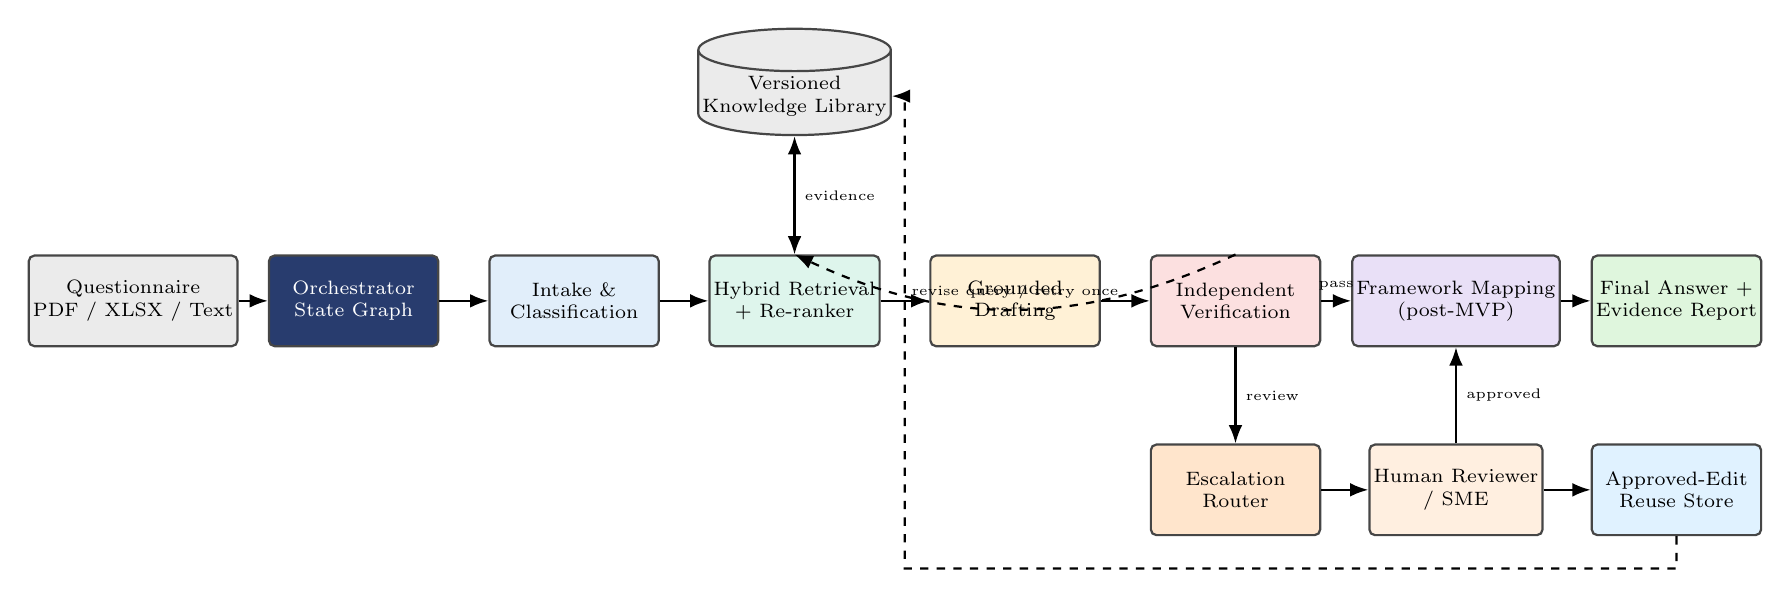
\begin{tikzpicture}[>=Latex, every node/.style={font=\scriptsize}]
\tikzset{agent/.style={draw=borderline,thick,rounded corners=2pt,align=center,
  minimum width=2.15cm,minimum height=1.15cm,inner sep=1.5pt,font=\scriptsize}}

\node[agent,fill=storecolor]                (inp)    at (0,0)    {Questionnaire\\PDF / XLSX / Text};
\node[agent,fill=orchcolor,text=white]      (orch)   at (2.8,0)  {Orchestrator\\State Graph};
\node[agent,fill=intakecolor]               (intake) at (5.6,0)  {Intake \&\\Classification};
\node[agent,fill=retrievalcolor]            (retr)   at (8.4,0)  {Hybrid Retrieval\\+ Re-ranker};
\node[agent,fill=draftcolor]                (draft)  at (11.2,0) {Grounded\\Drafting};
\node[agent,fill=verifycolor]               (verify) at (14.0,0) {Independent\\Verification};
\node[agent,fill=outputcolor]               (out)    at (19.6,0) {Final Answer +\\Evidence Report};

\node[draw=borderline,thick,cylinder,shape border rotate=90,aspect=0.22,
      fill=storecolor,minimum width=2.0cm,minimum height=1.35cm,align=center,
      inner sep=1.5pt,font=\scriptsize] (kl) at (8.4,2.6) {Versioned\\Knowledge Library};

\node[agent,fill=escalatecolor]     (esc) at (14.0,-2.4) {Escalation\\Router};
\node[agent,fill=escalatecolor!60]  (hr)  at (16.8,-2.4) {Human Reviewer\\/ SME};
\node[agent,fill=mapcolor]           (map) at (16.8,0) {Framework Mapping\\(post-MVP)};
\node[agent,fill=learncolor]         (learn) at (19.6,-2.4) {Approved-Edit\\Reuse Store};

\draw[->,thick] (inp.east)--(orch.west);
\draw[->,thick] (orch.east)--(intake.west);
\draw[->,thick] (intake.east)--(retr.west);
\draw[->,thick] (retr.east)--(draft.west);
\draw[->,thick] (draft.east)--(verify.west);
\draw[<->,thick] (retr.north)--(kl.south) node[midway,right,font=\tiny]{evidence};
\draw[->,thick] (verify.east)--(map.west) node[midway,above,font=\tiny]{pass};
\draw[->,thick] (map.east)--(out.west);
\draw[->,thick] (verify.south)--(esc.north) node[midway,right,font=\tiny]{review};
\draw[->,thick] (esc.east)--(hr.west);
\draw[->,thick] (hr.north)--(map.south) node[midway,right,font=\tiny]{approved};
\draw[->,thick] (hr.east)--(learn.west);
\draw[dashed,->,thick] (learn.south)--(19.6,-3.4)--(9.8,-3.4)--(9.8,2.6)--(kl.east);
\draw[dashed,->,thick,bend left=25] (verify.north) to node[midway,above,font=\tiny]{revise query / retry once} (retr.north);
\end{tikzpicture}}
\caption{Tentative Trustilo architecture. The core MVP is ingestion, retrieval, grounded drafting, independent verification, escalation, and human review. Framework mapping is shown as a post-MVP extension.}
\label{fig:architecture}
\end{figure}

\subsection{Agent Responsibilities}
\textbf{Orchestrator:} maintains per-question state, retries, configuration/version IDs, and audit events.\\
\textbf{Intake/Classification:} parses document structure, normalizes questions, classifies domain and expected answer type, and estimates duplicate/novelty similarity.\\
\textbf{Retrieval:} performs tenant-filtered dense+sparse retrieval, re-ranking, and evidence-version filtering.\\
\textbf{Drafting:} receives only selected evidence and emits a structured answer with claim-level citations or an abstention.\\
\textbf{Verification:} independently checks support/contradiction/freshness and can request one query rewrite/retrieval retry.\\
\textbf{Escalation:} routes cases using frozen thresholds and reason codes.\\
\textbf{Human Reviewer:} is the authoritative decision maker for escalated cases.\\
\textbf{Approved-Edit Reuse:} stores reviewer-approved answers as versioned retrieval exemplars; this is not autonomous online fine-tuning in the MVP.\\
\textbf{Framework Mapping (post-MVP):} suggests auditable mappings after the answer is finalized; mappings begin as human-confirmed suggestions.

\subsection{Requirement Updates Introduced by the Literature Review}
The literature review changes the initial proposal in five important ways:
\begin{enumerate}[leftmargin=1.7em]
    \item \textbf{Verification can trigger re-retrieval.} CoV-RAG shows that some errors begin with the query/retrieval step, so verification is not terminal \cite{he2024covrag}.
    \item \textbf{Evaluation is decomposed.} RAGAS/ARES motivate separate context relevance, faithfulness, and answer relevance measures rather than one aggregate score \cite{es2024ragas,saadfalcon2024ares}.
    \item \textbf{A small human gold set is mandatory.} Automated judges are useful for iteration but the final security-domain claims require SME review.
    \item \textbf{Hard negatives are deliberately created.} PrivacyQA augmentation and the Trustilo use case both require learning/evaluating on missing, misleading, and contradictory evidence, not only positive matches \cite{parvez2023privacyqa}.
    \item \textbf{Full compliance mapping is deferred.} Compliance RAG appears feasible, but it is a distinct research problem with structured representations and separate evaluation \cite{sun2025compliance}; it should not distract from validating the MVP grounding and verification loop.
\end{enumerate}

% ============================================================================
\section{Evaluation Plan}
% ============================================================================

\subsection{Metrics}
\begin{table}[H]
\centering
\caption{Evaluation Metrics}
\small
\begin{tabularx}{\textwidth}{L{0.22\textwidth}L{0.24\textwidth}Y}
\toprule
\textbf{Area} & \textbf{Metric} & \textbf{Interpretation} \\
\midrule
Ingestion & question extraction precision/recall or row accuracy & Whether the source questionnaire is normalized without dropping/misaligning questions. \\
Retrieval & Recall@5/10, MRR or nDCG & Whether gold supporting evidence appears high in the retrieved set. \\
Answer quality & SME correctness / substantive correction rate & Whether the final semantic answer is correct for the customer evidence. \\
Groundedness & claim-support precision/recall; unsupported-claim rate & Whether claims are entailed/supported by cited evidence. \\
RAG quality & context relevance, answer faithfulness, answer relevance & Component-level metrics inspired by RAGAS/ARES \cite{es2024ragas,saadfalcon2024ares}. \\
Verification & precision/recall/F1 on injected unsupported/contradictory cases & Whether the verifier catches known failures. \\
Escalation & precision, recall, F1; workload reduction & Whether risky cases reach humans without flagging nearly everything. \\
Calibration & Brier score and reliability diagram / ECE & Whether reported confidence aligns with observed correctness. \\
Operations & median/P95 latency, tokens/API cost & Practical speed and cost per question/questionnaire. \\
Human factors & reviewer time per question; acceptance/edit/reject rates & Whether automation actually reduces expert effort. \\
\bottomrule
\end{tabularx}
\end{table}

\subsection{Test Protocol}
The final benchmark should be stratified by question domain, duplicate/novel status, evidence sufficiency, and deliberate failure type. Prompt/model/retrieval changes are tuned only on the development split. Final thresholds are frozen before the held-out test. At least a subset of test cases should be independently reviewed twice or adjudicated when reviewers disagree, because ambiguous security wording can make a single label unreliable.

\subsection{Error Taxonomy}
Every failed final answer should be assigned a primary cause: ingestion/parsing error; retrieval miss; retrieved evidence insufficient; evidence stale; generator ignored evidence; unsupported synthesis; contradiction missed; verifier false positive; verifier false negative; escalation threshold error; or human-label ambiguity. This converts the final report from a single score into an engineering roadmap.

% ============================================================================
\section{Security, Auditability, and Data Governance}
% ============================================================================
Trustilo handles sensitive security posture information, so platform security is part of the product requirement rather than an afterthought. The MVP design includes tenant/customer namespace enforcement before retrieval; encryption in transit and at rest in the intended deployment; least-privilege service credentials; secrets management; versioned evidence with source/owner/date; immutable or append-oriented audit records for key decisions; configurable retention/deletion for test data; and prompt-injection defenses that treat uploaded documents as untrusted content rather than executable instructions. Any production deployment would require a separate threat model and security review beyond this academic prototype.

For framework references, NIST CSF 2.0 is a useful public mapping taxonomy and is organized around six Functions: Govern, Identify, Protect, Detect, Respond, and Recover \cite{nist2024csf,nist2024news}. CSA CAIQ/CCM provides a directly questionnaire-oriented cloud-security artifact. Proprietary or licensed standards content should only be stored/used according to the applicable license; the academic prototype can use identifiers, public descriptions, and customer-authorized material where appropriate.

% ============================================================================
\section{Proposed Technology Stack}
% ============================================================================
\begin{table}[H]
\centering
\caption{Candidate MVP Technology Stack}
\small
\begin{tabularx}{\textwidth}{L{0.21\textwidth}Y}
\toprule
\textbf{Layer} & \textbf{Candidate Approach} \\
\midrule
Backend/API & Python web API and background task workers. \\
Orchestration & Explicit graph/state-machine workflow with persisted per-question state and retry policies. \\
Parsing & XLSX/CSV parser; PDF text/table extraction with OCR only where necessary; deterministic normalization before LLM use. \\
Retrieval & PostgreSQL/pgvector or another vector store plus BM25/full-text search and an optional cross-encoder reranker. \\
LLM layer & Provider-abstracted model interface; stronger model for drafting/verification, smaller model where classification is sufficient. \\
Evidence storage & Object store for source files; relational metadata with customer namespace, version, source, and validity fields. \\
Reviewer console & Lightweight web UI focused on escalated claims, evidence, and approve/edit/reject actions. \\
Evaluation & Fixed JSONL/DB benchmark, experiment configuration IDs, RAGAS/ARES-inspired metrics plus SME gold labels. \\
Observability & Structured logs/traces, latency/token/cost accounting, and version IDs for model, prompts, retriever, and index. \\
\bottomrule
\end{tabularx}
\end{table}

% ============================================================================
\section{Timeline}
\label{sec:timeline}
% ============================================================================
\begin{figure}[H]
\centering
\resizebox{\textwidth}{!}{%
\begin{ganttchart}[
  vgrid,hgrid,x unit=0.34cm,y unit chart=0.48cm,y unit title=0.58cm,
  bar height=0.6,bar/.append style={fill=orchcolor},bar label font=\scriptsize,
  title label font=\bfseries\scriptsize,milestone label font=\scriptsize\itshape,
  milestone/.append style={fill=verifycolor},title/.style={draw=none,fill=storecolor}
]{1}{24}
\gantttitle{Trustilo Project Week}{24} \\
\gantttitlelist{1,...,24}{1} \\
\ganttbar{Requirement + literature review}{1}{4} \\
\ganttbar{Dataset schema + synthetic corpus}{3}{7} \\
\ganttbar{B0/B1 baseline implementation}{5}{8} \\
\ganttbar{Ingestion + classification}{7}{10} \\
\ganttbar{Hybrid retrieval + reranking}{9}{13} \\
\ganttbar{Grounded drafting}{12}{15} \\
\ganttbar{Verification + retry path}{14}{18} \\
\ganttbar{Escalation + reviewer console}{17}{20} \\
\ganttmilestone{End-to-end MVP}{20} \\
\ganttbar{Ablations + threshold calibration}{19}{22} \\
\ganttbar{Held-out test + SME pilot}{21}{23} \\
\ganttbar{Documentation + final report}{22}{24} \\
\ganttmilestone{Final submission}{24}
\end{ganttchart}}
\caption{Proposed 24-week schedule prioritizing the evidence-grounding and verification hypothesis before post-MVP features.}
\label{fig:gantt}
\end{figure}

% ============================================================================
\section{Expected Research Contributions and Deliverables}
% ============================================================================
The project is expected to deliver: (1) a reproducible security-questionnaire benchmark built from public questions plus a synthetic/versioned evidence library and SME labels; (2) a working multi-agent MVP; (3) a direct-LLM and single-agent RAG baseline; (4) ablation results quantifying the value of hybrid retrieval, verification, and escalation; (5) a reviewer console and audit trail; (6) a documented failure taxonomy; and (7) evidence showing whether the system reduces expert review effort at an acceptable groundedness level. A negative or mixed result is still useful if it clearly identifies which stage limits performance.

% ============================================================================
\section{Conclusion}
% ============================================================================
Trustilo should be evaluated primarily as an evidence-management and controlled-decision pipeline, not as a fluent text generator. The literature consistently points to the same design lesson: retrieval, generation, verification, and evaluation are distinct failure surfaces. The revised project therefore narrows the MVP to a measurable loop of \emph{retrieve $\rightarrow$ draft $\rightarrow$ verify $\rightarrow$ escalate/review}, supported by versioned evidence and explicit auditability. Compliance mapping and broader GRC automation remain valuable extensions only after that core loop demonstrates reliable groundedness on a held-out security-questionnaire benchmark.

% ============================================================================
\appendices
\section{Template Coverage Checklist}
\begin{table}[H]
\centering
\caption{Coverage of the Supplied AIF Templates}
\small
\begin{tabularx}{\textwidth}{L{0.36\textwidth}Y}
\toprule
\textbf{Template Item} & \textbf{Location in This Report} \\
\midrule
Project summary, problem, goals, applications, justification, limitations, assumptions, team & Section I \\
Expected inputs/outputs; end-user, functional, non-functional requirements; priority; success criteria & Section II \\
Data identification, sources, acquisition, challenges, baseline, resources & Section III \\
Research question and sub-problems; major ideas, datasets, models, issues & Section IV-A--IV-F \\
At least five detailed paper reviews with DOI/link, data, models, code, procedure, techniques, metrics, learning & Section IV-G (nine papers) \\
Literature review matrix & Section IV-H / Table~\ref{tab:litmatrix} \\
Project solution proposal and updated requirements from literature & Section V \\
Tentative architecture diagram & Fig.~\ref{fig:architecture} \\
Evaluation/experiment design & Sections V and VI \\
References in consistent style & Bibliography below \\
\bottomrule
\end{tabularx}
\end{table}

% ============================================================================
\begin{thebibliography}{99}

\bibitem{lewis2020rag}
P. Lewis, E. Perez, A. Piktus, \textit{et al.}, ``Retrieval-Augmented Generation for Knowledge-Intensive NLP Tasks,'' in \textit{Advances in Neural Information Processing Systems}, vol. 33, 2020. [Online]. Available: \url{https://proceedings.neurips.cc/paper/2020/hash/6b493230-Abstract.html}

\bibitem{he2024covrag}
B. He, N. Chen, X. He, L. Yan, Z. Wei, J. Luo, and Z.-H. Ling, ``Retrieving, Rethinking and Revising: The Chain-of-Verification Can Improve Retrieval Augmented Generation,'' in \textit{Findings of EMNLP 2024}, pp. 10371--10393, 2024, doi: 10.18653/v1/2024.findings-emnlp.607.

\bibitem{sun2025compliance}
J. Sun, Z. Luo, and Y. Li, ``A Compliance Checking Framework Based on Retrieval Augmented Generation,'' in \textit{Proceedings of the 31st International Conference on Computational Linguistics}, pp. 2603--2615, 2025. [Online]. Available: \url{https://aclanthology.org/2025.coling-main.178/}

\bibitem{es2024ragas}
S. Es, J. James, L. Espinosa Anke, and S. Schockaert, ``RAGAs: Automated Evaluation of Retrieval Augmented Generation,'' in \textit{Proceedings of the 18th EACL: System Demonstrations}, pp. 150--158, 2024, doi: 10.18653/v1/2024.eacl-demo.16.

\bibitem{saadfalcon2024ares}
J. Saad-Falcon, O. Khattab, C. Potts, and M. Zaharia, ``ARES: An Automated Evaluation Framework for Retrieval-Augmented Generation Systems,'' in \textit{Proceedings of NAACL-HLT}, pp. 338--354, 2024, doi: 10.18653/v1/2024.naacl-long.20.

\bibitem{dhuliawala2024cove}
S. Dhuliawala, M. Komeili, J. Xu, R. Raileanu, X. Li, A. Celikyilmaz, and J. Weston, ``Chain-of-Verification Reduces Hallucination in Large Language Models,'' in \textit{Findings of ACL 2024}, pp. 3563--3578, 2024, doi: 10.18653/v1/2024.findings-acl.212.

\bibitem{manakul2023selfcheckgpt}
P. Manakul, A. Liusie, and M. Gales, ``SelfCheckGPT: Zero-Resource Black-Box Hallucination Detection for Generative Large Language Models,'' in \textit{Proceedings of EMNLP}, pp. 9004--9017, 2023, doi: 10.18653/v1/2023.emnlp-main.557.

\bibitem{parvez2023privacyqa}
M. R. Parvez, J. Chi, W. U. Ahmad, Y. Tian, and K.-W. Chang, ``Retrieval Enhanced Data Augmentation for Question Answering on Privacy Policies,'' in \textit{Proceedings of EACL}, pp. 201--210, 2023, doi: 10.18653/v1/2023.eacl-main.16.

\bibitem{madaan2023selfrefine}
A. Madaan, N. Tandon, P. Gupta, \textit{et al.}, ``Self-Refine: Iterative Refinement with Self-Feedback,'' in \textit{Advances in Neural Information Processing Systems}, vol. 36, 2023, doi: 10.52202/075280-2019.

\bibitem{csa2026ccm}
Cloud Security Alliance, ``Cloud Controls Matrix and CAIQ v4.1,'' Jan. 27, 2026. [Online]. Available: \url{https://cloudsecurityalliance.org/artifacts/cloud-controls-matrix-v4-1}

\bibitem{csa2026guide}
Cloud Security Alliance, ``Introductory Guidance to Cloud Controls Matrix (CCM),'' Feb. 13, 2026. [Online]. Available: \url{https://cloudsecurityalliance.org/artifacts/introductory-guidance-to-ccm}

\bibitem{csa2026lite}
Cloud Security Alliance, ``CCM-Lite and CAIQ-Lite,'' Jan. 27, 2026. [Online]. Available: \url{https://cloudsecurityalliance.org/artifacts/ccm-lite-and-caiq-lite-v4}

\bibitem{nist2024csf}
National Institute of Standards and Technology, \textit{The NIST Cybersecurity Framework (CSF) 2.0}, NIST CSWP 29, Feb. 2024, doi: 10.6028/NIST.CSWP.29.

\bibitem{nist2024news}
National Institute of Standards and Technology, ``NIST Releases Version 2.0 of Landmark Cybersecurity Framework,'' Feb. 26, 2024. [Online]. Available: \url{https://www.nist.gov/news-events/news/2024/02/nist-releases-version-20-landmark-cybersecurity-framework}

\end{thebibliography}

\end{document}
